\documentclass
[answers]
{exam}

\linespread{1.1}

\usepackage{amsmath, amssymb, amsthm}  %% 數學符號用txfonts
\usepackage{mathrsfs} 
%\usepackage{pstricks,pstricks-add} % 引入 pstricks 和 pstricks-add 套件 (繪圖套件) 
%插入GGB圖片===================================
\usepackage{pgf,tikz}
\usepackage{mathrsfs}
\usetikzlibrary{arrows}
%=============================================
\usepackage{graphicx}   %% 插入圖片用
\usepackage{float}  %%強制插入圖片位置
\usepackage{caption}
\usepackage{subfigure}
\usepackage{color}
%\usepackage{minitoc}   %chapter下的小目錄
\usepackage{colortbl}
\usepackage{nopageno}
\usepackage{cases}
\usepackage{textcomp}             % for \textcelsius
\renewcommand{\arraystretch}{1.2} % 將表格行間距加大為原來的 1.2 倍
\arrayrulewidth=1pt               % 調整線條粗細為 1pt
\tabcolsep=15pt                   % 調整欄間距為 24pt


%\begin{figure}[h]
%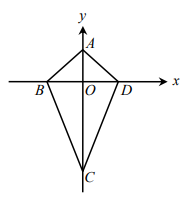
\includegraphics[scale=1.2]{./figure/2.png}
%\end{figure}

\usepackage{wrapfig}  %%圖文並排

%\begin{wrapfigure}{r}{6cm}  r:圖片靠右  6cm:離右邊6cm
%	\centering  圖片在右邊區塊的中間
%	\includegraphics[scale=0.6]{./figure/19.png}
%\end{wrapfigure}

\usepackage{tcolorbox}  %% 顏色方框
\usepackage{tikz}  %%繪製流程圖、腦圖...
\usepackage{array}  %%陣列
\usepackage{booktabs} %調整表格線與上下內容的間隔
\usepackage{multirow}
\usepackage{enumitem}
%可改enumerate的label
\usepackage{tasks}  %%選擇題
\settasks{label=(\Alph*),
		  label-width=3.5ex,
		  label-offset={0.4em},
		  label-align=left,
		  column-sep={1pt},
		  item-indent={21pt}, %%選項前後
		  before-skip={-0.7em},
		  after-skip={-0.7em}}
%[label=(\Alph*),label-width=4ex]  
%\Alph* 選項ABCD  \alph* 選項abcd  \arabic* 選項1234 \roman*羅馬數字
\usepackage{framed}  %%框框
%出入單行字加框  \framebox[\width]{我是一段话}

%插入圖片 \rightline{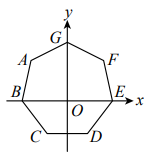
\includegraphics[scale=1.2]{./chapter_1/figure/1.png}}
\usepackage{diagbox}  %%斜線表格頭
\usepackage{ulem}
%\sout{文字} 刪除線		\uwave{文字} 波浪線
%\xout{文字} 斜刪除線		\uuline{文字} 雙下划線
\usepackage[margin=2cm]{geometry} %邊界設定
\usepackage[export]{adjustbox} %插入圖片
\usepackage[colorlinks=true,linkcolor=blue]{hyperref}
%%[是否開啟目錄顏色,目錄顏色設定]{超連結}

%\usepackage{fancyhdr}  %%這兩行是頁首頁尾
%\pagestyle{fancy}  %%頁首頁尾格式
%\fancypagestyle{plain}{}
%\renewcommand{\headrulewidth}{0.4pt}  %%頁首下方直線厚度
%\cfoot{觀念解數學--~\thepage~--態度解人生}
%\fancyhead{} % 清除所有頁首設定
%\fancyhead[RO,LE]{\thechapter}
%\fancyfoot{} % 清除所有頁尾設定
%\fancyfoot[LE,RO]{第~\thepage~頁}      % 頁碼放在偶數頁的左邊及奇數頁的右邊
%\fancyfoot[LO,CE]{奇數頁左及偶數頁中}
%\fancyfoot[CO,RE]{奇數頁中及偶數頁右}
% Texmaker使用者: 上方選擇XeLaTeX後再編譯
\usepackage{xeCJK}   % Chinese input settings
\setCJKmainfont{標楷體} % Windows使用者請使用這行
\setmainfont{Times New Roman}
\defaultCJKfontfeatures{AutoFakeBold=0.5,AutoFakeSlant=0} %以後不用再設定粗斜
\newCJKfontfamily\WC{華康行楷體W5}                       
\XeTeXlinebreaklocale "zh"
\XeTeXlinebreakskip = 0pt plus 1pt
%%上兩行才能讓中文自動換行
\makeatletter
\def\rightharpoonfill@{\arrowfill@\relbar\relbar\rightharpoonup}
\newcommand{\vect}{\mathpalette{\overarrow@\rightharpoonfill@}}
\makeatother
%向量

%\renewcommand{\qedsymbol}{}
\newcommand{\R}{\mathbb{R}} %mathbb 雙行粗體
\newcommand{\Z}{\mathbb{Z}}
\newcommand{\Q}{\mathbb{Q}}
\newcommand{\N}{\mathbb{N}}
\renewcommand{\S}{\mathbb{S}}
\newcommand{\f}{\ensuremath{\mathcal{F}}} 
%%\ensuremath  非數學模式自動加上$符號
\newcommand\norm[1]{\left\lVert#1\right\rVert}
\newcommand\abs[1]{\left| #1\right| }
\newcommand\ul[1]{\uline{\hspace*{#1}}}
\newcommand\px{\mathrel{/\mkern-5mu/}}  %平行
%文繞圖 wrapfigure 和 條列式環境 item 並列, 需在 enumerate 環境之中
%\itemwrap{<先用 \begin{wrapfigure} 環境插入圖片, 再接著文字>}
\newcommand{\itemwrap}[1]{
	\item \parbox[t]{\dimexpr\textwidth-\leftmargin}{
		\vspace{-3.2mm}#1}}

%\itemwraps{<需縮排的行數>}{<圖片寬度(配合上面寬度)>}{<文字>}
\newcommand{\itemwraps}[3]{
	\item \parbox[t]{\dimexpr\textwidth-\leftmargin}{%
		\vspace{-3.2mm}
		\begin{wrapfigure}[#1]{r}{#2}
		\end{wrapfigure}#3}}


\newif\ifqr\qrfalse %QR
\newcommand{\qr}[1]{\ifqr\relax\else #1\fi} 
%教用學生版 %一鍵隱藏答案  \true隱藏  \false顯示

\newif\ifans\ansfalse
\newcommand{\ans}[1]{\ifans\relax\else\framebox{#1}\fi} 

\DeclareMathOperator{\sign}{sign} %sign為非斜體

\parindent=0pt  %%首行空格
\renewcommand{\qedsymbol}{}  %證明後面沒方格

%\theoremstyle{remark}
%\newtheorem{prop}{Proposition}
%\newtheorem{thm}[prop]{Theorem}   %% 編號跟著 prop 走
%\newtheorem*{thm}{Theorem}   %% 有自己的編號
%\newtheorem{lem}{\underline{Lemma}}
%\newtheorem*{rmk}{\bf{\underline{Remark}}}
%\newtheorem*{ex}{\underline{Examples}}
%\newtheorem{cor}{Corollary}
%\newtheorem*{coro}{Corollary}
%\newtheorem{lem}[thm]{Lemma}
\theoremstyle{definition}
%\newtheorem*{defn}{Definition}
\newtheorem{foc}{\WC\underline{\Large{焦點}}}[section]
\newtheorem*{pra}{\WC\underline{\Large{隨堂小練}}}
\newtheorem*{hw}{\WC\underline{\Large{課後練功坊}}}
\newtheorem*{suyu}{\WC\underline{\Large{素養挑戰題}}}
%有*是無編號  無*是有編號
% Authur information
%\title{標題}
%\author{作者}
%\date{日期}

%\begin{document}
%\renewcommand{\qedsymbol}{}  %證明後面沒方格
%\maketitle   %此功能為是否顯示title
%\fontsize{20pt}{25pt}\selectfont  %%目錄字體大小
%\tableofcontents  %%目錄

%\fontsize{12pt}{25pt}\selectfon


%===================================================================

\title{{\Huge{\WC{第一冊習題詳解本}}}}
\author{}
\date{}

\begin{document}

%\fontsize{20pt}{25pt}\selectfont  %%目錄字體大小
%\tableofcontents  %目錄
\let\cleardoublepage\clearpage
\fontsize{12pt}{25pt}\selectfont  %%內文字體大小
\newpage
%-----------------------------------------------------
\maketitle
\section{\WC{直線方程式}}
\subsection{~}
\subsubsection{直線方程式}
\begin{questions}
%linef_1
\question

設直線$L$的斜率為$3$,且在$x$軸的截距為$2$,求直線$L$的方程式為\ul{50pt}。
\\ \rightline{【明倫】}
\begin{solution}~\\
	$y = 3x - 6$
\end{solution}

%linef_2
\question

設直線$L$通過兩點$\left( 3,2\right)$、$\left( 4,-1\right)$,則$L$的方程式為\ul{50pt}。
\\ \rightline{【中女中】}
\begin{solution}~\\
	$3x + y - 11 = 0$
\end{solution}

$ $\\$ $\\
%linef_3
\question

設直線$L$通過點$\left( 4,1\right)$ 且$y$截距為$5$,求$L$的直線方程式為\ul{50pt}。
\\ \rightline{【三民】}
\begin{solution}~\\
	$x + y = 5$
\end{solution}

%linef_4
\question

$A\left( -2,3\right)$、$B\left( 1,9\right)$,求過點$\left( 1,2\right)$且平行$\overline{AB}$的直線方程式為\ul{50pt}。
\\ \rightline{【屏中】}
\begin{solution}~\\
	$2x - y = 0$
\end{solution}

%linef_5
\question

過$x+2y=3$與$2x-y=1$之交點且與$3x-y+6=0$平行之線性方程式為\ul{50pt}。
\\ \rightline{【豐原】}
\begin{solution}~\\
	$3x - y - 2 = 0$
\end{solution}

$ $\\$ $\\$ $\\$ $\\
%linef_6
\question

一直線$L_1$過$\left( 1,3\right($、$\left( 2,-1\right($兩點,另一直線$L_2$過$\left( 3,-2  \right)$且與$L_1$垂直,則直線$L_2$的方程式為\ul{50pt}
\\ \rightline{【屏中】}
\begin{solution}~\\
	$y + 2 = \dfrac{1}{4} \left( x-3 \right)$
\end{solution}

%linef_7
\question

設直線$L$過$17x+11y+5=0$與$13x+23y+9=0$的交點,且$L$與直線$x-3y+2=0$垂直,則$L$的方程式為\ul{50pt}
\\ \rightline{【延平】}
\begin{solution}~\\
	$x + y = - \dfrac{17}{31}$
\end{solution}

%linef_8
\question

$\triangle ABC$中,已知$A\left( 2,0\right($,且$D\left( 3,4\right)$、$E\left( 6,5\right)$分別為$\overline{AB}$與$\overline{BC}$之中點,若直線$AC$的方程式為$ax-by-2=0$其中$a,b$均為整數,則數對$\left( a,b \right)=$\ul{50pt}。
\\ \rightline{【華江】}
\begin{solution}~\\
	$\left( 1,3 \right)$
\end{solution}

%linef_9
\question

\begin{minipage}[t]{0.7\linewidth}
	如圖,$O$為座標原點,直線$L$與$x$軸、$y$軸分別交於$A$與$B$兩點,已知$\overline{OA}=2\overline{OB}$且直線$L$過點$C\left( 1,1\right)$,則$L$的方程式為\ul{50pt}
\end{minipage}
\hfill
\begin{minipage}[t]{0.3\linewidth}
	\vspace*{-0.3cm}
	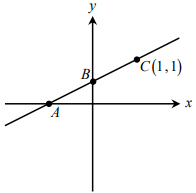
\includegraphics[scale=1]{./chapter_3/figure/10.png}
	\raggedleft %靠右對齊
\end{minipage}
\\ \rightline{【三民】}
\begin{solution}~\\
	$x-2y+1=0$
\end{solution}

%linef_10
\question

請選出斜率最小的直線:
\begin{tasks}(3)
	\task $2x+y+1=0$
	\task $3x-4y+5=0$
	\task $y-3=8\left( x+1\right)$
	\task $y=5x-7$
	\task $\dfrac{x}{2}+\dfrac{y}{3}=1$
\end{tasks}
\rightline{【成淵】}
\begin{solution}~\\
	(A)
\end{solution}

%linef_11
\question

\begin{minipage}[t]{0.7\linewidth}
	坐標平面上四條直線$L_1$、$L_2$、$L_3$、$L_4$與$x$軸、$y$軸及直線$y=x$的相關位置如圖所示,其中$L_1$與$L_3$垂直,而$L_3$與$L_4$平行。設$L_1$、$L_2$、$L_3$、$L_4$的方程式分別為$y=m_1x$,$y=m_2x$,$y=m_3x$以及$y=m_4x+c$。試問下列哪些選項是正確的?
\end{minipage}
\hfill
\begin{minipage}[t]{0.3\linewidth}
	\vspace*{-0.3cm}
	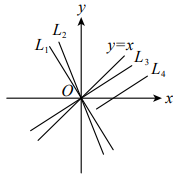
\includegraphics[scale=1]{./chapter_3/figure/11.png}
	\raggedleft %靠右對齊
\end{minipage}


\begin{tasks}(3)
	\tasks $m_3 > m_2 > m_1$
	\tasks $m_1 \cdot m_4 = -1$
	\tasks $m_1 < -1$
	\tasks $m_2 \cdot m_3 < -1$
	\tasks $c > 0$
\end{tasks}
\rightline{【98學測】}
\begin{solution}~\\
	(B)(C)(D)
\end{solution}

%linef_12
\question

\begin{minipage}[t]{0.7\linewidth}
	如圖,三直線的方程式依次為$L_1:y=a_1x+b_1$,$L_2:y=a_2x+b_2$,$L_3:y=a_3x+b_3$,下列選項何者正確?
\end{minipage}
\hfill
\begin{minipage}[t]{0.3\linewidth}
	\vspace*{-0.3cm}
	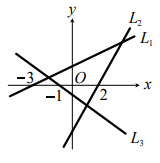
\includegraphics[scale=1]{./chapter_3/figure/12.png}
	\raggedleft %靠右對齊
\end{minipage}


\begin{tasks}(5)
	\task $a_1 > a_2$
	\task $b_2 > b_3$
	\task $a_1b_2 > a_2b_2$
	\task $2a_3 > b_3$
	\task $a_2 + b_2 < 0$。
\end{tasks}
\rightline{【松山】}
\begin{solution}~\\
	(C)(E)
\end{solution}

%linef_13
\question

\begin{minipage}[t]{0.7\linewidth}
	如圖,$L_1:y=ax+b$,$L_2:y=cx+d$,$L_3:y=ex+f$,下列各數哪一個最小?
\end{minipage}
\hfill
\begin{minipage}[t]{0.3\linewidth}
	\vspace*{-0.3cm}
	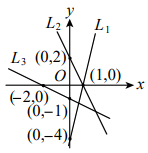
\includegraphics[scale=1]{./chapter_3/figure/13.png}
	\raggedleft %靠右對齊
\end{minipage}

\begin{tasks}(5)
	\task $a$
	\task $b$
	\task $c$
	\task $d$
	\task $e$
\end{tasks}
\rightline{【中山】}
\begin{solution}~\\
	(B)
\end{solution}


$ $\\$ $\\$ $\\$ $\\$ $\\$ $\\

%linef_14
\question

\begin{minipage}[t]{0.7\linewidth}
	如圖,,三直線$L_1:y=m_1x+b_1$,$L_2:y=m_2x+b_2$,$L_3:y=m_3x+b_3$,下列有關$m_1$、$m_2$、$m_3$、$b_1$、$b_2$、$b_3$之選項,何者正確?
\end{minipage}
\hfill
\begin{minipage}[t]{0.3\linewidth}
	\vspace*{-0.3cm}
	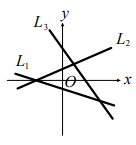
\includegraphics[scale=1]{./chapter_3/figure/14.png}
	\raggedleft %靠右對齊
\end{minipage}

\begin{tasks}(3)
	\task $m_3<m_1<m_2$
	\task $m_1<m_2<m_3$
	\task $b_2>b_3>b_1$
	\task $b_3>b_2>b_1$
	\task $b_1>b_2>b_3$
\end{tasks}
\rightline{【雄中】}
\begin{solution}~\\
	(A)(D)
\end{solution}


%linef_15
\question

(1)不論$m$為任何實數,直線$L:y=mx-m+3$恆過定點$P$,求$P$座標為\ul{50pt}。\\
(2)承(1),已知$A\left( -1,-3\right)$、$B\left( 4,2\right)$,若$L$與$\overline{AB}$相交,求$m$的範圍為\ul{50pt}。
\\ \rightline{【景美】}
\begin{solution}~\\
	(1)$ \left(  1,3 \right)$(2)$m \leq - \dfrac{1}{3} \vee m \geq 3$
\end{solution}

%linef_16
\question

已知直線$L:mx-y+3-m=0$與兩點$A\left( -2,-3\right)$、$B\left( 3,2\right)$,若$L$與$\overline{AB}$不相交,試求實數$m$的範圍為\ul{50pt}。
\\ \rightline{【中女中】}
\begin{solution}~\\
	$-\dfrac{1}{2} < m < 2$
\end{solution}

%linef_17
\question

設$A\left( 1,5\right)$、$B\left( 4,1\right)$、$C\left( 2,-1\right)$,直線$L:mx-2m-y+6=0$,若直線$L$與$\triangle ABC$有交點,求$m$的最大可能範圍為\ul{50pt}。
\\ \rightline{【竹北】}
\begin{solution}~\\
		$m \leq - \dfrac{5}{2} \vee m \geq 1$
\end{solution}

%linef_18
\question

$\triangle ABC$三邊所在的直線為$2x+y-3=0$、$y=0$、$x-y=0$,若直線$y=mx+3$與$\triangle ABC$相交,則$m$可能為下列何數?

\begin{tasks}(5)
	\task $-\dfrac{1}{3}$
	\task $ -5$
	\task $-2$
	\task $\dfrac{5}{2}$
	\task $1$
\end{tasks}
\rightline{【屏女】}
\begin{solution}~\\
	(B)(C)
\end{solution}

%linef_19
\question

令$A\left( 1,0\right)$、$B\left( 1,1\right)$、$\left( -1,1\right)$、$D\left( -1,0\right)$,若直線$y=mx+3$恆與長方形$ABCD$有交點,則$m$的值可能為?

\begin{tasks}(5)
	\task $0$
	\task $1$
	\task $2$
	\task $-3$
	\task $-4$
\end{tasks}
\rightline{【中崙】}

\begin{solution}~\\
	(C)(D)(E)
\end{solution}

$ $\\$ $\\

%linef_20
\question

座標平面中,設$A\left( -5,0\right)$與$B\left( -2,3\right)$,若直線$L:3x-4y+k=0$與$\overline{AB}$相交,則實數$k$的範圍是\ul{50pt}。
\\ \rightline{【華江】}
\begin{solution}~\\
	$15 \leq k \leq 18$
\end{solution}

%linef_21
\question

座標平面三點$A\left( 3,4\right)$、$B\left( -2,-5\right)$、$C\left( 7,0\right)$,過$B$點將$\triangle ABC$的面積等分的直線方程式為\ul{50pt}。
\\ \rightline{【三民】}
\begin{solution}~\\
	$x-y=3$
\end{solution}

%linef_22
\question

某直線通過點$\left( 7,4\right)$,且將平行四邊形$ABCD$之面積平分,若$A\left( 1,1\right)$、$B\left( 3,4\right)$、$C\left( 9,5\right)$、$D\left( 7,2\right)$為平行四邊形$ABCD$的四個頂點,求直線方程式為\ul{50pt}。
\\ \rightline{【成功】}
\begin{solution}~\\
	$x-2y+1=0$
\end{solution}

$ $\\$ $\\
%linef_23
\question

已知點$A\left( 9,-2\right)$,點$B\left( -1,8\right)$,直線$L:x-2y+7=0$,若$Q$為$L$上使$\angle AQB$為直角的點,求$Q$點座標為\ul{50pt}。
\\ \rightline{【建中】}
\begin{solution}~\\
	$\left( -3,2 \right) \vee \left( 9,8 \right)$
\end{solution}

%linef_24
\question

已知$A\left( 4,6\right)$、$B\left( 8,2\right)$、$C\left( 5,-7\right)$,$\overline{AB}$邊上的高所在的直線方程式為\ul{50pt}。
\\ \rightline{【板中】}
\begin{solution}~\\
	$x-y-12=0$
\end{solution}

%linef_25
\question

$A\left( 1,2\right)$、$B\left( 5,-2\right)$為座標平面上的兩點,則$\overline{AB}$之中垂線方程式為\ul{50pt}。
\\ \rightline{【北一】}
\begin{solution}~\\
	$x-y=3$
\end{solution}

$ $\\$ $\\$ $\\$ $\\
%linef_26
\question

已知平面上$A\left( 1,3\right)$、$B\left( -2,2\right)$兩點,若$P$點在$x$軸上,且$\overline{PA}=\overline{PB}$,則$P$點座標為\ul{50pt}。
\\ \rightline{【前鎮】}
\begin{solution}~\\
	$\left( \dfrac{1}{3} ,0\right)$
\end{solution}

%linef_27
\question

鳶形$ABCD$(其中$\overline{AB}=\overline{AD}$、$\overline{CB}=\overline{CD}$),已知$A\left( 2,-1\right)$、$B\left( 2,1\right)$、$C\left( -2,3\right)$,求$D$點座標為\ul{50pt}
\\ \rightline{【松山】}
\begin{solution}~\\
	$\left( 0,-1 \right)$
\end{solution}

%linef_28
\question

已知平行四邊形的兩邊所在直線方程式為$2x+y=18$及$x-y=-6$,且一頂點為$\left( 3,-6\right)$,求此平行四邊形在第二象限上的頂點座標為\ul{50pt},
\\ \rightline{【景美】}
\begin{solution}~\\
	$\left( -2,4 \right)$
\end{solution}
$ $\\$ $\\
%linef_29
\question

一平行四邊形兩邊分別在直線$2x-y+2=0$及$x+3y-6=0$上,其中一頂點為$\left( 2,-1\right)$,則此平行四邊形之周長為\ul{50pt}。
\\ \rightline{【新店】}
\begin{solution}~\\
	$2\sqrt{5}+2\sqrt{10}$
\end{solution}

%linef_30
\question

一直線$L$通過點$\left( -3,2\right)$,若$L$的$x$截距與$y$截距恰為相反數且皆為非0實數,則直線$L$的方程式為\ul{50pt}
\\ \rightline{【中女中】}
\begin{solution}~\\
	$x-y+5=0$
\end{solution}


%linef_31
\question

若有一直線在坐標軸上之$x$截距與$y$截距相等且通點$\left( -4,2\right)$,則直線方程式為\ul{50pt}。
\\ \rightline{【基中】}
\begin{solution}~\\
	$x+2y=0 \vee x+y+2=0$
\end{solution}

$ $\\$ $\\
%linef_32
\question

設直線$L$通過點$\left( -2,3\right)$且與$x$軸、$y$軸截距的絕對值相等,則$L$之方程式為\ul{50pt}。
\\ \rightline{【高師】}
\begin{solution}~\\
	$3x+2y=0 \vee x+y = 1 \vee x - y = -5$
\end{solution}

%linef_33
\question

求截距和為$3$與$2x-y+4=0$垂直的直線方程式為\ul{50pt}。
\\ \rightline{【附中】}
\begin{solution}~\\
	$x+2y = 2$
\end{solution}

%linef_34
\question

設一直線$L$與$4x+5y+7=0$垂直,且$L$的兩截距和為$4$,若$L$的方程式為$x+by+c=0$,則數對$\left( b,c\right)=$\ul{50pt}。
\\ \rightline{【雄女】}
\begin{solution}~\\
	$\left( -\dfrac{4}{5},16\right)$
\end{solution}
$ $\\$ $\\$ $\\
%linef_35
\question

若直線$L$通過點$\left( 9,8\right)$,且直線$L$與兩座標軸所圍成的區域面積為$3$,則直線$L$的直線方程式為\ul{50pt}。
\\ \rightline{【延平】}
\begin{solution}~\\
	$32x-27y-72=0 \vee 2x-3y+6=0 $
\end{solution}

%linef_36
\question

一直線在第三象限內與兩軸所圍成之三角形面積為$6$,已知此直線的斜率為$-\dfrac{1}{3}$,求此直線方程式為\ul{50pt}。
\\ \rightline{【松山】}
\begin{solution}~\\
	$x+3y+6=0$
\end{solution}

%linef_37
\question

設直線$L$的斜率是$\dfrac{3}{2}$,且與兩座標軸所圍成的三角形面積為$12$,求$L$的方程式為\ul{50pt}。
\\ \rightline{【北一】}
\begin{solution}~\\
	$3x-2y=12 \vee 3x-2y = -12$
\end{solution}
$ $\\$ $\\$ $\\
%linef_38
\question

設直線$L$過$\left( 3,-5\right)$且與兩座標軸於第四象限所形成的三角面積為最小時,試求:\\
(1)直線$L$的方程式為\ul{50pt}。(請化為$ax+by+c=0$的形式)\\
(2)此最小的三角形面積為\ul{50pt}\\
\\ \rightline{【中女中】}
\begin{solution}~\\
	(1)$5x-3y = 30$(2)$30$
\end{solution}

%linef_39
\question

平面上有一定點$P\left( 1,1\right)$,一直線$L$過$P$點且與$x$軸、$y$軸分別交流於$A$、$B$兩點($L$不經過原點),原點為$O$,則此三點所形成的三角形$OAB$,\\
(1)求在第一象限所圍成的三角形$OAB$的面積的最小值$t=$\ul{50pt}及當時直線$L$的方程式為\ul{50pt}。\\
(2)若三角形$OAB$的面積為$4$,則滿足此種條件之直線$L$的方程式為\ul{50pt}
\\ \rightline{【建中】}
\begin{solution}~\\
	(1)$2$;$x+y-2=0$(2)$\left( 2 + \sqrt{2}\right) x + \left( 2-\sqrt{2}\right) y -4=0$或$\left( 2 - \sqrt{2}\right) x + \left( 2+\sqrt{2}\right) y -4=0$或$\left( -2 + \sqrt{6}\right) x + \left( -2 -\sqrt{6}\right) y +4=0$或$\left( -2 - \sqrt{6}\right) x + \left( -2 +\sqrt{6}\right) y +4=0$
\end{solution}

\end{questions}

\end{document}
